\documentclass[twoside]{book}

% Packages required by doxygen
\usepackage{calc}
\usepackage{doxygen}
\usepackage{graphicx}
\usepackage[utf8]{inputenc}
\usepackage{makeidx}
\usepackage{multicol}
\usepackage{multirow}
\usepackage{textcomp}
\usepackage[table]{xcolor}

% Font selection
\usepackage[T1]{fontenc}
\usepackage{mathptmx}
\usepackage[scaled=.90]{helvet}
\usepackage{courier}
\usepackage{amssymb}
\usepackage{sectsty}
\renewcommand{\familydefault}{\sfdefault}
\allsectionsfont{%
  \fontseries{bc}\selectfont%
  \color{darkgray}%
}
\renewcommand{\DoxyLabelFont}{%
  \fontseries{bc}\selectfont%
  \color{darkgray}%
}

% Page & text layout
\usepackage{geometry}
\geometry{%
  a4paper,%
  top=2.5cm,%
  bottom=2.5cm,%
  left=2.5cm,%
  right=2.5cm%
}
\tolerance=750
\hfuzz=15pt
\hbadness=750
\setlength{\emergencystretch}{15pt}
\setlength{\parindent}{0cm}
\setlength{\parskip}{0.2cm}
\makeatletter
\renewcommand{\paragraph}{%
  \@startsection{paragraph}{4}{0ex}{-1.0ex}{1.0ex}{%
    \normalfont\normalsize\bfseries\SS@parafont%
  }%
}
\renewcommand{\subparagraph}{%
  \@startsection{subparagraph}{5}{0ex}{-1.0ex}{1.0ex}{%
    \normalfont\normalsize\bfseries\SS@subparafont%
  }%
}
\makeatother

% Headers & footers
\usepackage{fancyhdr}
\pagestyle{fancyplain}
\fancyhead[LE]{\fancyplain{}{\bfseries\thepage}}
\fancyhead[CE]{\fancyplain{}{}}
\fancyhead[RE]{\fancyplain{}{\bfseries\leftmark}}
\fancyhead[LO]{\fancyplain{}{\bfseries\rightmark}}
\fancyhead[CO]{\fancyplain{}{}}
\fancyhead[RO]{\fancyplain{}{\bfseries\thepage}}
\fancyfoot[LE]{\fancyplain{}{}}
\fancyfoot[CE]{\fancyplain{}{}}
\fancyfoot[RE]{\fancyplain{}{\bfseries\scriptsize Generated on Sun Mar 2 2014 23\-:49\-:42 for O\-M\-P2\-D Java by Doxygen }}
\fancyfoot[LO]{\fancyplain{}{\bfseries\scriptsize Generated on Sun Mar 2 2014 23\-:49\-:42 for O\-M\-P2\-D Java by Doxygen }}
\fancyfoot[CO]{\fancyplain{}{}}
\fancyfoot[RO]{\fancyplain{}{}}
\renewcommand{\footrulewidth}{0.4pt}
\renewcommand{\chaptermark}[1]{%
  \markboth{#1}{}%
}
\renewcommand{\sectionmark}[1]{%
  \markright{\thesection\ #1}%
}

% Indices & bibliography
\usepackage{natbib}
\usepackage[titles]{tocloft}
\setcounter{tocdepth}{3}
\setcounter{secnumdepth}{5}
\makeindex

% Hyperlinks (required, but should be loaded last)
\usepackage{ifpdf}
\ifpdf
  \usepackage[pdftex,pagebackref=true]{hyperref}
\else
  \usepackage[ps2pdf,pagebackref=true]{hyperref}
\fi
\hypersetup{%
  colorlinks=true,%
  linkcolor=blue,%
  citecolor=blue,%
  unicode%
}

% Custom commands
\newcommand{\clearemptydoublepage}{%
  \newpage{\pagestyle{empty}\cleardoublepage}%
}


%===== C O N T E N T S =====

\begin{document}

% Titlepage & ToC
\hypersetup{pageanchor=false}
\pagenumbering{roman}
\begin{titlepage}
\vspace*{7cm}
\begin{center}%
{\Large O\-M\-P2\-D Java }\\
\vspace*{1cm}
{\large Generated by Doxygen 1.8.6}\\
\vspace*{0.5cm}
{\small Sun Mar 2 2014 23:49:42}\\
\end{center}
\end{titlepage}
\clearemptydoublepage
\tableofcontents
\clearemptydoublepage
\pagenumbering{arabic}
\hypersetup{pageanchor=true}

%--- Begin generated contents ---
\chapter{Namespace Index}
\section{Packages}
Here are the packages with brief descriptions (if available)\-:\begin{DoxyCompactList}
\item\contentsline{section}{\hyperlink{namespaceOMP2D}{O\-M\-P2\-D} }{\pageref{namespaceOMP2D}}{}
\end{DoxyCompactList}

\chapter{Hierarchical Index}
\section{Class Hierarchy}
This inheritance list is sorted roughly, but not completely, alphabetically\-:\begin{DoxyCompactList}
\item \contentsline{section}{O\-M\-P2\-D.\-Cuda\-Director}{\pageref{classOMP2D_1_1CudaDirector}}{}
\item Exception\begin{DoxyCompactList}
\item \contentsline{section}{O\-M\-P2\-D.\-Bad\-Dimensions\-Exception}{\pageref{classOMP2D_1_1BadDimensionsException}}{}
\end{DoxyCompactList}
\item \contentsline{section}{O\-M\-P2\-D.\-Matrix}{\pageref{classOMP2D_1_1Matrix}}{}
\begin{DoxyCompactList}
\item \contentsline{section}{O\-M\-P2\-D.\-Cuda\-Matrix}{\pageref{classOMP2D_1_1CudaMatrix}}{}
\item \contentsline{section}{O\-M\-P2\-D.\-Dictionary\-X}{\pageref{classOMP2D_1_1DictionaryX}}{}
\item \contentsline{section}{O\-M\-P2\-D.\-Dictionary\-Y}{\pageref{classOMP2D_1_1DictionaryY}}{}
\end{DoxyCompactList}
\item \contentsline{section}{O\-M\-P2\-D.\-O\-M\-P2\-D}{\pageref{classOMP2D_1_1OMP2D}}{}
\item \contentsline{section}{image\-J\-O\-M\-P2\-D\-Plugin.\-O\-M\-P2\-D\-Plugin\-Test}{\pageref{classimageJOMP2DPlugin_1_1OMP2DPluginTest}}{}
\item \contentsline{section}{test\-O\-M\-P2\-D.\-Test\-Matrix}{\pageref{classtestOMP2D_1_1TestMatrix}}{}
\item Plug\-In\-Filter\begin{DoxyCompactList}
\item \contentsline{section}{image\-J\-O\-M\-P2\-D\-Plugin.\-O\-M\-P2\-D\-\_\-\-Plugin}{\pageref{classimageJOMP2DPlugin_1_1OMP2D__Plugin}}{}
\end{DoxyCompactList}
\item Pointer\begin{DoxyCompactList}
\item \contentsline{section}{O\-M\-P2\-D.\-Clever\-Pointer$<$ V $>$}{\pageref{classOMP2D_1_1CleverPointer_3_01V_01_4}}{}
\end{DoxyCompactList}
\end{DoxyCompactList}

\chapter{Class Index}
\section{Class List}
Here are the classes, structs, unions and interfaces with brief descriptions\-:\begin{DoxyCompactList}
\item\contentsline{section}{\hyperlink{classOMP2D_1_1MatrixOperations_1_1IncompatibleDimensionsException}{O\-M\-P2\-D.\-Matrix\-Operations.\-Incompatible\-Dimensions\-Exception} }{\pageref{classOMP2D_1_1MatrixOperations_1_1IncompatibleDimensionsException}}{}
\item\contentsline{section}{\hyperlink{classOMP2D_1_1MatrixOperations}{O\-M\-P2\-D.\-Matrix\-Operations} }{\pageref{classOMP2D_1_1MatrixOperations}}{}
\item\contentsline{section}{\hyperlink{classOMP2D_1_1OMP2D}{O\-M\-P2\-D.\-O\-M\-P2\-D} }{\pageref{classOMP2D_1_1OMP2D}}{}
\item\contentsline{section}{\hyperlink{classOMP2D_1_1PursuitFunctions}{O\-M\-P2\-D.\-Pursuit\-Functions} }{\pageref{classOMP2D_1_1PursuitFunctions}}{}
\end{DoxyCompactList}

\chapter{File Index}
\section{File List}
Here is a list of all files with brief descriptions\-:\begin{DoxyCompactList}
\item\contentsline{section}{/home/matt/cuda-\/workspace/\-O\-M\-P2\-D Java/src/\-O\-M\-P2\-D/\hyperlink{MatrixOperations_8java}{Matrix\-Operations.\-java} }{\pageref{MatrixOperations_8java}}{}
\item\contentsline{section}{/home/matt/cuda-\/workspace/\-O\-M\-P2\-D Java/src/\-O\-M\-P2\-D/\hyperlink{OMP2D_8java}{O\-M\-P2\-D.\-java} }{\pageref{OMP2D_8java}}{}
\item\contentsline{section}{/home/matt/cuda-\/workspace/\-O\-M\-P2\-D Java/src/\-O\-M\-P2\-D/\hyperlink{PursuitFunctions_8java}{Pursuit\-Functions.\-java} }{\pageref{PursuitFunctions_8java}}{}
\end{DoxyCompactList}

\chapter{Namespace Documentation}
\hypertarget{namespaceOMP2D}{\section{Package O\-M\-P2\-D}
\label{namespaceOMP2D}\index{O\-M\-P2\-D@{O\-M\-P2\-D}}
}
\subsection*{Classes}
\begin{DoxyCompactItemize}
\item 
class \hyperlink{classOMP2D_1_1BadDimensionsException}{Bad\-Dimensions\-Exception}
\item 
class \hyperlink{classOMP2D_1_1CleverPointer_3_01V_01_4}{Clever\-Pointer$<$ V $>$}
\item 
class \hyperlink{classOMP2D_1_1CudaDirector}{Cuda\-Director}
\item 
class \hyperlink{classOMP2D_1_1CudaMatrix}{Cuda\-Matrix}
\item 
class \hyperlink{classOMP2D_1_1DictionaryX}{Dictionary\-X}
\item 
class \hyperlink{classOMP2D_1_1DictionaryY}{Dictionary\-Y}
\item 
class \hyperlink{classOMP2D_1_1Matrix}{Matrix}
\item 
class \hyperlink{classOMP2D_1_1OMP2D}{O\-M\-P2\-D}
\end{DoxyCompactItemize}

\chapter{Class Documentation}
\hypertarget{classOMP2D_1_1MatrixOperations_1_1IncompatibleDimensionsException}{\section{O\-M\-P2\-D.\-Matrix\-Operations.\-Incompatible\-Dimensions\-Exception Class Reference}
\label{classOMP2D_1_1MatrixOperations_1_1IncompatibleDimensionsException}\index{O\-M\-P2\-D.\-Matrix\-Operations.\-Incompatible\-Dimensions\-Exception@{O\-M\-P2\-D.\-Matrix\-Operations.\-Incompatible\-Dimensions\-Exception}}
}
Inheritance diagram for O\-M\-P2\-D.\-Matrix\-Operations.\-Incompatible\-Dimensions\-Exception\-:\begin{figure}[H]
\begin{center}
\leavevmode
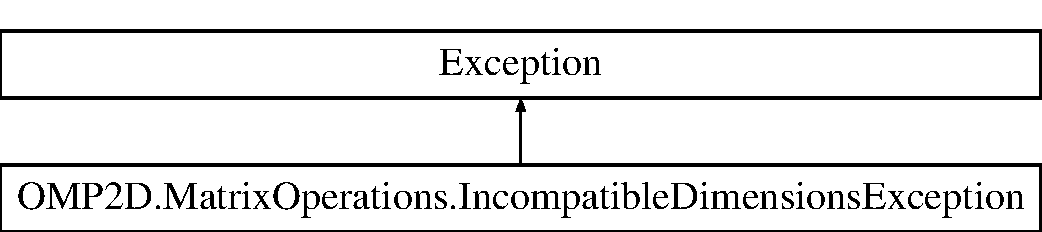
\includegraphics[height=2.000000cm]{classOMP2D_1_1MatrixOperations_1_1IncompatibleDimensionsException}
\end{center}
\end{figure}
\subsection*{Public Member Functions}
\begin{DoxyCompactItemize}
\item 
\hyperlink{classOMP2D_1_1MatrixOperations_1_1IncompatibleDimensionsException_a0e5a16dc4643385797385418e494d309}{Incompatible\-Dimensions\-Exception} (String msg)
\item 
\hyperlink{classOMP2D_1_1MatrixOperations_1_1IncompatibleDimensionsException_aae52cccef243d78d596309dd46d084b2}{Incompatible\-Dimensions\-Exception} ()
\item 
\hyperlink{classOMP2D_1_1MatrixOperations_1_1IncompatibleDimensionsException_a1d8c5075cfc4c1a2efda645ac3b48ec4}{Incompatible\-Dimensions\-Exception} (String msg, int expected, int actual)
\end{DoxyCompactItemize}


\subsection{Constructor \& Destructor Documentation}
\hypertarget{classOMP2D_1_1MatrixOperations_1_1IncompatibleDimensionsException_a0e5a16dc4643385797385418e494d309}{\index{O\-M\-P2\-D\-::\-Matrix\-Operations\-::\-Incompatible\-Dimensions\-Exception@{O\-M\-P2\-D\-::\-Matrix\-Operations\-::\-Incompatible\-Dimensions\-Exception}!Incompatible\-Dimensions\-Exception@{Incompatible\-Dimensions\-Exception}}
\index{Incompatible\-Dimensions\-Exception@{Incompatible\-Dimensions\-Exception}!OMP2D::MatrixOperations::IncompatibleDimensionsException@{O\-M\-P2\-D\-::\-Matrix\-Operations\-::\-Incompatible\-Dimensions\-Exception}}
\subsubsection[{Incompatible\-Dimensions\-Exception}]{\setlength{\rightskip}{0pt plus 5cm}O\-M\-P2\-D.\-Matrix\-Operations.\-Incompatible\-Dimensions\-Exception.\-Incompatible\-Dimensions\-Exception (
\begin{DoxyParamCaption}
\item[{String}]{msg}
\end{DoxyParamCaption}
)}}\label{classOMP2D_1_1MatrixOperations_1_1IncompatibleDimensionsException_a0e5a16dc4643385797385418e494d309}
\hypertarget{classOMP2D_1_1MatrixOperations_1_1IncompatibleDimensionsException_aae52cccef243d78d596309dd46d084b2}{\index{O\-M\-P2\-D\-::\-Matrix\-Operations\-::\-Incompatible\-Dimensions\-Exception@{O\-M\-P2\-D\-::\-Matrix\-Operations\-::\-Incompatible\-Dimensions\-Exception}!Incompatible\-Dimensions\-Exception@{Incompatible\-Dimensions\-Exception}}
\index{Incompatible\-Dimensions\-Exception@{Incompatible\-Dimensions\-Exception}!OMP2D::MatrixOperations::IncompatibleDimensionsException@{O\-M\-P2\-D\-::\-Matrix\-Operations\-::\-Incompatible\-Dimensions\-Exception}}
\subsubsection[{Incompatible\-Dimensions\-Exception}]{\setlength{\rightskip}{0pt plus 5cm}O\-M\-P2\-D.\-Matrix\-Operations.\-Incompatible\-Dimensions\-Exception.\-Incompatible\-Dimensions\-Exception (
\begin{DoxyParamCaption}
{}
\end{DoxyParamCaption}
)}}\label{classOMP2D_1_1MatrixOperations_1_1IncompatibleDimensionsException_aae52cccef243d78d596309dd46d084b2}
\hypertarget{classOMP2D_1_1MatrixOperations_1_1IncompatibleDimensionsException_a1d8c5075cfc4c1a2efda645ac3b48ec4}{\index{O\-M\-P2\-D\-::\-Matrix\-Operations\-::\-Incompatible\-Dimensions\-Exception@{O\-M\-P2\-D\-::\-Matrix\-Operations\-::\-Incompatible\-Dimensions\-Exception}!Incompatible\-Dimensions\-Exception@{Incompatible\-Dimensions\-Exception}}
\index{Incompatible\-Dimensions\-Exception@{Incompatible\-Dimensions\-Exception}!OMP2D::MatrixOperations::IncompatibleDimensionsException@{O\-M\-P2\-D\-::\-Matrix\-Operations\-::\-Incompatible\-Dimensions\-Exception}}
\subsubsection[{Incompatible\-Dimensions\-Exception}]{\setlength{\rightskip}{0pt plus 5cm}O\-M\-P2\-D.\-Matrix\-Operations.\-Incompatible\-Dimensions\-Exception.\-Incompatible\-Dimensions\-Exception (
\begin{DoxyParamCaption}
\item[{String}]{msg, }
\item[{int}]{expected, }
\item[{int}]{actual}
\end{DoxyParamCaption}
)}}\label{classOMP2D_1_1MatrixOperations_1_1IncompatibleDimensionsException_a1d8c5075cfc4c1a2efda645ac3b48ec4}


The documentation for this class was generated from the following file\-:\begin{DoxyCompactItemize}
\item 
/home/matt/cuda-\/workspace/\-O\-M\-P2\-D Java/src/\-O\-M\-P2\-D/\hyperlink{MatrixOperations_8java}{Matrix\-Operations.\-java}\end{DoxyCompactItemize}

\hypertarget{classOMP2D_1_1MatrixOperations}{\section{O\-M\-P2\-D.\-Matrix\-Operations Class Reference}
\label{classOMP2D_1_1MatrixOperations}\index{O\-M\-P2\-D.\-Matrix\-Operations@{O\-M\-P2\-D.\-Matrix\-Operations}}
}
\subsection*{Classes}
\begin{DoxyCompactItemize}
\item 
class \hyperlink{classOMP2D_1_1MatrixOperations_1_1IncompatibleDimensionsException}{Incompatible\-Dimensions\-Exception}
\end{DoxyCompactItemize}
\subsection*{Static Public Member Functions}
\begin{DoxyCompactItemize}
\item 
static double \hyperlink{classOMP2D_1_1MatrixOperations_a0ffd0bed3beb6b14b1e6c80259fdb2fc}{real\-Inner\-Product} (double\mbox{[}$\,$\mbox{]} vector1, double\mbox{[}$\,$\mbox{]} vector2)  throws Incompatible\-Dimensions\-Exception 
\item 
static double\mbox{[}$\,$\mbox{]} \hyperlink{classOMP2D_1_1MatrixOperations_a9f4c857451b167cc252827d17cd1413c}{normalize} (double\mbox{[}$\,$\mbox{]} vector, double norm\-Vector)
\item 
static double\mbox{[}$\,$\mbox{]} \hyperlink{classOMP2D_1_1MatrixOperations_a435ecf7d2a5c1dff9f70ef542b17804b}{normalize} (double\mbox{[}$\,$\mbox{]} vector)  throws Incompatible\-Dimensions\-Exception 
\item 
static double \hyperlink{classOMP2D_1_1MatrixOperations_ad4e2f7e46255b1af0dc78b06151ce0a1}{norm} (double\mbox{[}$\,$\mbox{]} vector)  throws Incompatible\-Dimensions\-Exception 
\item 
static double\mbox{[}$\,$\mbox{]} \hyperlink{classOMP2D_1_1MatrixOperations_a4fbee19c7844db28af5203a2b6087206}{add\-Vectors} (double\mbox{[}$\,$\mbox{]} vector1, double\mbox{[}$\,$\mbox{]} vector2, double scalar)  throws Incompatible\-Dimensions\-Exception 
\item 
static double\mbox{[}$\,$\mbox{]} \hyperlink{classOMP2D_1_1MatrixOperations_aaeb17605f361eadab3ffb12918d24496}{add\-Vectors} (double\mbox{[}$\,$\mbox{]} vector1, double\mbox{[}$\,$\mbox{]} vector2)  throws Incompatible\-Dimensions\-Exception 
\item 
static double\mbox{[}$\,$\mbox{]} \hyperlink{classOMP2D_1_1MatrixOperations_aaa1507cc4bd3d390fea146ab29abb5bf}{multiply\-Matrix\-Vector} (double\mbox{[}$\,$\mbox{]}\mbox{[}$\,$\mbox{]} matrix, double\mbox{[}$\,$\mbox{]} vector, char thing)  throws Incompatible\-Dimensions\-Exception 
\item 
static double\mbox{[}$\,$\mbox{]} \hyperlink{classOMP2D_1_1MatrixOperations_af63d77a6ef1d2bae746c7f47099f01ed}{scale\-Vector} (double\mbox{[}$\,$\mbox{]} vector, double factor)
\item 
static double\mbox{[}$\,$\mbox{]}\mbox{[}$\,$\mbox{]} \hyperlink{classOMP2D_1_1MatrixOperations_a3f7a1739a39b7bc42567c8011694bb5f}{outer\-Product} (double\mbox{[}$\,$\mbox{]}\mbox{[}$\,$\mbox{]} matrix, double\mbox{[}$\,$\mbox{]} vector, double\mbox{[}$\,$\mbox{]} vector\-Scalar)  throws Incompatible\-Dimensions\-Exception 
\item 
static double\mbox{[}$\,$\mbox{]} \hyperlink{classOMP2D_1_1MatrixOperations_aee29169db5db03e194c041f89399b35c}{kron\-Atom} (double\mbox{[}$\,$\mbox{]} vector1, double\mbox{[}$\,$\mbox{]} vector2)  throws Incompatible\-Dimensions\-Exception 
\item 
static double \hyperlink{classOMP2D_1_1MatrixOperations_a20c8df75f73908438dd418cb803d077e}{max\-Abs} (double\mbox{[}$\,$\mbox{]} vector)
\item 
static double \hyperlink{classOMP2D_1_1MatrixOperations_a3326a590f1c188296d0e14cd6f5476ad}{max\-Abs} (double\mbox{[}$\,$\mbox{]}\mbox{[}$\,$\mbox{]} matrix)
\item 
static void \hyperlink{classOMP2D_1_1MatrixOperations_a9dfd3ba69faf8f5c905a5c9dcac30cdd}{allocate\-Elements} (double\mbox{[}$\,$\mbox{]} vector, double value, int num)
\item 
static double\mbox{[}$\,$\mbox{]}\mbox{[}$\,$\mbox{]} \hyperlink{classOMP2D_1_1MatrixOperations_a66a0e1bf820558880db67d2efac229cb}{matrix\-Multiply} (double\mbox{[}$\,$\mbox{]}\mbox{[}$\,$\mbox{]} matrix1, double\mbox{[}$\,$\mbox{]}\mbox{[}$\,$\mbox{]} matrix2, char thing1, char thing2)  throws Incompatible\-Dimensions\-Exception 
\item 
static double \hyperlink{classOMP2D_1_1MatrixOperations_aa2f4938d53dcbb632fbf2e499705f29f}{vector\-Matrix\-Vector} (double\mbox{[}$\,$\mbox{]} vector1, double\mbox{[}$\,$\mbox{]}\mbox{[}$\,$\mbox{]} matrix, double\mbox{[}$\,$\mbox{]} vector2)  throws Incompatible\-Dimensions\-Exception 
\end{DoxyCompactItemize}


\subsection{Member Function Documentation}
\hypertarget{classOMP2D_1_1MatrixOperations_a4fbee19c7844db28af5203a2b6087206}{\index{O\-M\-P2\-D\-::\-Matrix\-Operations@{O\-M\-P2\-D\-::\-Matrix\-Operations}!add\-Vectors@{add\-Vectors}}
\index{add\-Vectors@{add\-Vectors}!OMP2D::MatrixOperations@{O\-M\-P2\-D\-::\-Matrix\-Operations}}
\subsubsection[{add\-Vectors}]{\setlength{\rightskip}{0pt plus 5cm}static double \mbox{[}$\,$\mbox{]} O\-M\-P2\-D.\-Matrix\-Operations.\-add\-Vectors (
\begin{DoxyParamCaption}
\item[{double\mbox{[}$\,$\mbox{]}}]{vector1, }
\item[{double\mbox{[}$\,$\mbox{]}}]{vector2, }
\item[{double}]{scalar}
\end{DoxyParamCaption}
) throws {\bf Incompatible\-Dimensions\-Exception}\hspace{0.3cm}{\ttfamily [static]}}}\label{classOMP2D_1_1MatrixOperations_a4fbee19c7844db28af5203a2b6087206}
Adds and scales the first vector T\-O\-D\-O This should be handle outside this class 
\begin{DoxyParams}{Parameters}
{\em vector1} & \\
\hline
{\em vector2} & \\
\hline
{\em scalar} & \\
\hline
\end{DoxyParams}
\begin{DoxyReturn}{Returns}

\end{DoxyReturn}

\begin{DoxyExceptions}{Exceptions}
{\em \hyperlink{classOMP2D_1_1MatrixOperations_1_1IncompatibleDimensionsException}{Incompatible\-Dimensions\-Exception}} & \\
\hline
\end{DoxyExceptions}
\hypertarget{classOMP2D_1_1MatrixOperations_aaeb17605f361eadab3ffb12918d24496}{\index{O\-M\-P2\-D\-::\-Matrix\-Operations@{O\-M\-P2\-D\-::\-Matrix\-Operations}!add\-Vectors@{add\-Vectors}}
\index{add\-Vectors@{add\-Vectors}!OMP2D::MatrixOperations@{O\-M\-P2\-D\-::\-Matrix\-Operations}}
\subsubsection[{add\-Vectors}]{\setlength{\rightskip}{0pt plus 5cm}static double \mbox{[}$\,$\mbox{]} O\-M\-P2\-D.\-Matrix\-Operations.\-add\-Vectors (
\begin{DoxyParamCaption}
\item[{double\mbox{[}$\,$\mbox{]}}]{vector1, }
\item[{double\mbox{[}$\,$\mbox{]}}]{vector2}
\end{DoxyParamCaption}
) throws {\bf Incompatible\-Dimensions\-Exception}\hspace{0.3cm}{\ttfamily [static]}}}\label{classOMP2D_1_1MatrixOperations_aaeb17605f361eadab3ffb12918d24496}
Adds two vectors of the same length together 
\begin{DoxyParams}{Parameters}
{\em vector1} & \\
\hline
{\em vector2} & \\
\hline
\end{DoxyParams}
\begin{DoxyReturn}{Returns}
The resulting vector 
\end{DoxyReturn}

\begin{DoxyExceptions}{Exceptions}
{\em \hyperlink{classOMP2D_1_1MatrixOperations_1_1IncompatibleDimensionsException}{Incompatible\-Dimensions\-Exception}} & \\
\hline
\end{DoxyExceptions}
\hypertarget{classOMP2D_1_1MatrixOperations_a9dfd3ba69faf8f5c905a5c9dcac30cdd}{\index{O\-M\-P2\-D\-::\-Matrix\-Operations@{O\-M\-P2\-D\-::\-Matrix\-Operations}!allocate\-Elements@{allocate\-Elements}}
\index{allocate\-Elements@{allocate\-Elements}!OMP2D::MatrixOperations@{O\-M\-P2\-D\-::\-Matrix\-Operations}}
\subsubsection[{allocate\-Elements}]{\setlength{\rightskip}{0pt plus 5cm}static void O\-M\-P2\-D.\-Matrix\-Operations.\-allocate\-Elements (
\begin{DoxyParamCaption}
\item[{double\mbox{[}$\,$\mbox{]}}]{vector, }
\item[{double}]{value, }
\item[{int}]{num}
\end{DoxyParamCaption}
)\hspace{0.3cm}{\ttfamily [static]}}}\label{classOMP2D_1_1MatrixOperations_a9dfd3ba69faf8f5c905a5c9dcac30cdd}
Fills a vector with a given value up the {\itshape n}-\/th element Not necessary in Java for we have Array.\-fill() 
\begin{DoxyParams}{Parameters}
{\em vector} & The vector to be filled \\
\hline
{\em value} & The value which will be inserted \\
\hline
{\em num} & The last numbered index which will be filled 0 to num inclusive \\
\hline
\end{DoxyParams}
\hypertarget{classOMP2D_1_1MatrixOperations_aee29169db5db03e194c041f89399b35c}{\index{O\-M\-P2\-D\-::\-Matrix\-Operations@{O\-M\-P2\-D\-::\-Matrix\-Operations}!kron\-Atom@{kron\-Atom}}
\index{kron\-Atom@{kron\-Atom}!OMP2D::MatrixOperations@{O\-M\-P2\-D\-::\-Matrix\-Operations}}
\subsubsection[{kron\-Atom}]{\setlength{\rightskip}{0pt plus 5cm}static double \mbox{[}$\,$\mbox{]} O\-M\-P2\-D.\-Matrix\-Operations.\-kron\-Atom (
\begin{DoxyParamCaption}
\item[{double\mbox{[}$\,$\mbox{]}}]{vector1, }
\item[{double\mbox{[}$\,$\mbox{]}}]{vector2}
\end{DoxyParamCaption}
) throws {\bf Incompatible\-Dimensions\-Exception}\hspace{0.3cm}{\ttfamily [static]}}}\label{classOMP2D_1_1MatrixOperations_aee29169db5db03e194c041f89399b35c}
Applies the Kronecker product of two vectors (Q\-U\-E\-S\-T\-I\-O\-N should this be matrices as well?) 
\begin{DoxyParams}{Parameters}
{\em vector1} & \\
\hline
{\em vector2} & \\
\hline
\end{DoxyParams}
\begin{DoxyReturn}{Returns}

\end{DoxyReturn}

\begin{DoxyExceptions}{Exceptions}
{\em \hyperlink{classOMP2D_1_1MatrixOperations_1_1IncompatibleDimensionsException}{Incompatible\-Dimensions\-Exception}} & \\
\hline
\end{DoxyExceptions}
\hypertarget{classOMP2D_1_1MatrixOperations_a66a0e1bf820558880db67d2efac229cb}{\index{O\-M\-P2\-D\-::\-Matrix\-Operations@{O\-M\-P2\-D\-::\-Matrix\-Operations}!matrix\-Multiply@{matrix\-Multiply}}
\index{matrix\-Multiply@{matrix\-Multiply}!OMP2D::MatrixOperations@{O\-M\-P2\-D\-::\-Matrix\-Operations}}
\subsubsection[{matrix\-Multiply}]{\setlength{\rightskip}{0pt plus 5cm}static double \mbox{[}$\,$\mbox{]}\mbox{[}$\,$\mbox{]} O\-M\-P2\-D.\-Matrix\-Operations.\-matrix\-Multiply (
\begin{DoxyParamCaption}
\item[{double}]{matrix1\mbox{[}$\,$\mbox{]}\mbox{[}$\,$\mbox{]}, }
\item[{double}]{matrix2\mbox{[}$\,$\mbox{]}\mbox{[}$\,$\mbox{]}, }
\item[{char}]{thing1, }
\item[{char}]{thing2}
\end{DoxyParamCaption}
) throws {\bf Incompatible\-Dimensions\-Exception}\hspace{0.3cm}{\ttfamily [static]}}}\label{classOMP2D_1_1MatrixOperations_a66a0e1bf820558880db67d2efac229cb}
Performs the dot product of two matrices 
\begin{DoxyParams}{Parameters}
{\em matrix1} & A matrix defined as $M^{x \times y}$ \\
\hline
{\em matrix2} & A matrix defined as $N^{y \times z}$ \\
\hline
{\em thing1} & (Q\-U\-E\-S\-T\-I\-O\-N not sure what this is) \\
\hline
{\em thing2} & \\
\hline
\end{DoxyParams}
\begin{DoxyReturn}{Returns}
The resulting matrix 
\end{DoxyReturn}

\begin{DoxyExceptions}{Exceptions}
{\em \hyperlink{classOMP2D_1_1MatrixOperations_1_1IncompatibleDimensionsException}{Incompatible\-Dimensions\-Exception}} & \\
\hline
\end{DoxyExceptions}
\hypertarget{classOMP2D_1_1MatrixOperations_a20c8df75f73908438dd418cb803d077e}{\index{O\-M\-P2\-D\-::\-Matrix\-Operations@{O\-M\-P2\-D\-::\-Matrix\-Operations}!max\-Abs@{max\-Abs}}
\index{max\-Abs@{max\-Abs}!OMP2D::MatrixOperations@{O\-M\-P2\-D\-::\-Matrix\-Operations}}
\subsubsection[{max\-Abs}]{\setlength{\rightskip}{0pt plus 5cm}static double O\-M\-P2\-D.\-Matrix\-Operations.\-max\-Abs (
\begin{DoxyParamCaption}
\item[{double\mbox{[}$\,$\mbox{]}}]{vector}
\end{DoxyParamCaption}
)\hspace{0.3cm}{\ttfamily [static]}}}\label{classOMP2D_1_1MatrixOperations_a20c8df75f73908438dd418cb803d077e}
Finds the largest absolute value of a given vector 
\begin{DoxyParams}{Parameters}
{\em vector} & \\
\hline
\end{DoxyParams}
\begin{DoxyReturn}{Returns}
the largest absolute value 
\end{DoxyReturn}
\hypertarget{classOMP2D_1_1MatrixOperations_a3326a590f1c188296d0e14cd6f5476ad}{\index{O\-M\-P2\-D\-::\-Matrix\-Operations@{O\-M\-P2\-D\-::\-Matrix\-Operations}!max\-Abs@{max\-Abs}}
\index{max\-Abs@{max\-Abs}!OMP2D::MatrixOperations@{O\-M\-P2\-D\-::\-Matrix\-Operations}}
\subsubsection[{max\-Abs}]{\setlength{\rightskip}{0pt plus 5cm}static double O\-M\-P2\-D.\-Matrix\-Operations.\-max\-Abs (
\begin{DoxyParamCaption}
\item[{double}]{matrix\mbox{[}$\,$\mbox{]}\mbox{[}$\,$\mbox{]}}
\end{DoxyParamCaption}
)\hspace{0.3cm}{\ttfamily [static]}}}\label{classOMP2D_1_1MatrixOperations_a3326a590f1c188296d0e14cd6f5476ad}
Finds the largest absolute value of a given matrix 
\begin{DoxyParams}{Parameters}
{\em matrix} & \\
\hline
\end{DoxyParams}
\begin{DoxyReturn}{Returns}

\end{DoxyReturn}
\hypertarget{classOMP2D_1_1MatrixOperations_aaa1507cc4bd3d390fea146ab29abb5bf}{\index{O\-M\-P2\-D\-::\-Matrix\-Operations@{O\-M\-P2\-D\-::\-Matrix\-Operations}!multiply\-Matrix\-Vector@{multiply\-Matrix\-Vector}}
\index{multiply\-Matrix\-Vector@{multiply\-Matrix\-Vector}!OMP2D::MatrixOperations@{O\-M\-P2\-D\-::\-Matrix\-Operations}}
\subsubsection[{multiply\-Matrix\-Vector}]{\setlength{\rightskip}{0pt plus 5cm}static double \mbox{[}$\,$\mbox{]} O\-M\-P2\-D.\-Matrix\-Operations.\-multiply\-Matrix\-Vector (
\begin{DoxyParamCaption}
\item[{double}]{matrix\mbox{[}$\,$\mbox{]}\mbox{[}$\,$\mbox{]}, }
\item[{double\mbox{[}$\,$\mbox{]}}]{vector, }
\item[{char}]{thing}
\end{DoxyParamCaption}
) throws {\bf Incompatible\-Dimensions\-Exception}\hspace{0.3cm}{\ttfamily [static]}}}\label{classOMP2D_1_1MatrixOperations_aaa1507cc4bd3d390fea146ab29abb5bf}
Multiplies a given matrix and vector 
\begin{DoxyParams}{Parameters}
{\em matrix} & A matrix of dimensions (m,n) \\
\hline
{\em vector} & A vector of dimension m \\
\hline
{\em thing} & (Q\-U\-E\-S\-T\-I\-O\-N I'm not sure what this is...) \\
\hline
\end{DoxyParams}
\begin{DoxyReturn}{Returns}
the resulting vector 
\end{DoxyReturn}

\begin{DoxyExceptions}{Exceptions}
{\em \hyperlink{classOMP2D_1_1MatrixOperations_1_1IncompatibleDimensionsException}{Incompatible\-Dimensions\-Exception}} & \\
\hline
\end{DoxyExceptions}
\hypertarget{classOMP2D_1_1MatrixOperations_ad4e2f7e46255b1af0dc78b06151ce0a1}{\index{O\-M\-P2\-D\-::\-Matrix\-Operations@{O\-M\-P2\-D\-::\-Matrix\-Operations}!norm@{norm}}
\index{norm@{norm}!OMP2D::MatrixOperations@{O\-M\-P2\-D\-::\-Matrix\-Operations}}
\subsubsection[{norm}]{\setlength{\rightskip}{0pt plus 5cm}static double O\-M\-P2\-D.\-Matrix\-Operations.\-norm (
\begin{DoxyParamCaption}
\item[{double\mbox{[}$\,$\mbox{]}}]{vector}
\end{DoxyParamCaption}
) throws {\bf Incompatible\-Dimensions\-Exception}\hspace{0.3cm}{\ttfamily [static]}}}\label{classOMP2D_1_1MatrixOperations_ad4e2f7e46255b1af0dc78b06151ce0a1}
Performs the Euclidean norm operation on a vector 
\begin{DoxyParams}{Parameters}
{\em vector} & \\
\hline
\end{DoxyParams}
\begin{DoxyReturn}{Returns}
The Euclidean norm 
\end{DoxyReturn}

\begin{DoxyExceptions}{Exceptions}
{\em \hyperlink{classOMP2D_1_1MatrixOperations_1_1IncompatibleDimensionsException}{Incompatible\-Dimensions\-Exception}} & \\
\hline
\end{DoxyExceptions}
\hypertarget{classOMP2D_1_1MatrixOperations_a9f4c857451b167cc252827d17cd1413c}{\index{O\-M\-P2\-D\-::\-Matrix\-Operations@{O\-M\-P2\-D\-::\-Matrix\-Operations}!normalize@{normalize}}
\index{normalize@{normalize}!OMP2D::MatrixOperations@{O\-M\-P2\-D\-::\-Matrix\-Operations}}
\subsubsection[{normalize}]{\setlength{\rightskip}{0pt plus 5cm}static double \mbox{[}$\,$\mbox{]} O\-M\-P2\-D.\-Matrix\-Operations.\-normalize (
\begin{DoxyParamCaption}
\item[{double\mbox{[}$\,$\mbox{]}}]{vector, }
\item[{double}]{norm\-Vector}
\end{DoxyParamCaption}
)\hspace{0.3cm}{\ttfamily [static]}}}\label{classOMP2D_1_1MatrixOperations_a9f4c857451b167cc252827d17cd1413c}
This is especially silly 
\begin{DoxyParams}{Parameters}
{\em vector} & \\
\hline
{\em norm\-Vector} & \\
\hline
\end{DoxyParams}
\begin{DoxyReturn}{Returns}

\end{DoxyReturn}
\hypertarget{classOMP2D_1_1MatrixOperations_a435ecf7d2a5c1dff9f70ef542b17804b}{\index{O\-M\-P2\-D\-::\-Matrix\-Operations@{O\-M\-P2\-D\-::\-Matrix\-Operations}!normalize@{normalize}}
\index{normalize@{normalize}!OMP2D::MatrixOperations@{O\-M\-P2\-D\-::\-Matrix\-Operations}}
\subsubsection[{normalize}]{\setlength{\rightskip}{0pt plus 5cm}static double \mbox{[}$\,$\mbox{]} O\-M\-P2\-D.\-Matrix\-Operations.\-normalize (
\begin{DoxyParamCaption}
\item[{double\mbox{[}$\,$\mbox{]}}]{vector}
\end{DoxyParamCaption}
) throws {\bf Incompatible\-Dimensions\-Exception}\hspace{0.3cm}{\ttfamily [static]}}}\label{classOMP2D_1_1MatrixOperations_a435ecf7d2a5c1dff9f70ef542b17804b}
Q\-U\-E\-S\-T\-I\-O\-N What is the purpose of this method given I already have norm 
\begin{DoxyParams}{Parameters}
{\em vector} & \\
\hline
\end{DoxyParams}
\begin{DoxyReturn}{Returns}

\end{DoxyReturn}

\begin{DoxyExceptions}{Exceptions}
{\em \hyperlink{classOMP2D_1_1MatrixOperations_1_1IncompatibleDimensionsException}{Incompatible\-Dimensions\-Exception}} & \\
\hline
\end{DoxyExceptions}
\hypertarget{classOMP2D_1_1MatrixOperations_a3f7a1739a39b7bc42567c8011694bb5f}{\index{O\-M\-P2\-D\-::\-Matrix\-Operations@{O\-M\-P2\-D\-::\-Matrix\-Operations}!outer\-Product@{outer\-Product}}
\index{outer\-Product@{outer\-Product}!OMP2D::MatrixOperations@{O\-M\-P2\-D\-::\-Matrix\-Operations}}
\subsubsection[{outer\-Product}]{\setlength{\rightskip}{0pt plus 5cm}static double \mbox{[}$\,$\mbox{]}\mbox{[}$\,$\mbox{]} O\-M\-P2\-D.\-Matrix\-Operations.\-outer\-Product (
\begin{DoxyParamCaption}
\item[{double}]{matrix\mbox{[}$\,$\mbox{]}\mbox{[}$\,$\mbox{]}, }
\item[{double\mbox{[}$\,$\mbox{]}}]{vector, }
\item[{double\mbox{[}$\,$\mbox{]}}]{vector\-Scalar}
\end{DoxyParamCaption}
) throws {\bf Incompatible\-Dimensions\-Exception}\hspace{0.3cm}{\ttfamily [static]}}}\label{classOMP2D_1_1MatrixOperations_a3f7a1739a39b7bc42567c8011694bb5f}
Performs the outer product 
\begin{DoxyParams}{Parameters}
{\em matrix} & A transposed vector \\
\hline
{\em vector} & \\
\hline
{\em vector\-Scalar} & T\-O\-D\-O this should be done outside this method \\
\hline
\end{DoxyParams}
\begin{DoxyReturn}{Returns}

\end{DoxyReturn}

\begin{DoxyExceptions}{Exceptions}
{\em \hyperlink{classOMP2D_1_1MatrixOperations_1_1IncompatibleDimensionsException}{Incompatible\-Dimensions\-Exception}} & \\
\hline
\end{DoxyExceptions}
\hypertarget{classOMP2D_1_1MatrixOperations_a0ffd0bed3beb6b14b1e6c80259fdb2fc}{\index{O\-M\-P2\-D\-::\-Matrix\-Operations@{O\-M\-P2\-D\-::\-Matrix\-Operations}!real\-Inner\-Product@{real\-Inner\-Product}}
\index{real\-Inner\-Product@{real\-Inner\-Product}!OMP2D::MatrixOperations@{O\-M\-P2\-D\-::\-Matrix\-Operations}}
\subsubsection[{real\-Inner\-Product}]{\setlength{\rightskip}{0pt plus 5cm}static double O\-M\-P2\-D.\-Matrix\-Operations.\-real\-Inner\-Product (
\begin{DoxyParamCaption}
\item[{double\mbox{[}$\,$\mbox{]}}]{vector1, }
\item[{double\mbox{[}$\,$\mbox{]}}]{vector2}
\end{DoxyParamCaption}
) throws {\bf Incompatible\-Dimensions\-Exception}\hspace{0.3cm}{\ttfamily [static]}}}\label{classOMP2D_1_1MatrixOperations_a0ffd0bed3beb6b14b1e6c80259fdb2fc}
Performs the inner product operation on two vectors 
\begin{DoxyParams}{Parameters}
{\em vector1} & \\
\hline
{\em vector2} & \\
\hline
\end{DoxyParams}
\begin{DoxyReturn}{Returns}
The inner product 
\end{DoxyReturn}

\begin{DoxyExceptions}{Exceptions}
{\em \hyperlink{classOMP2D_1_1MatrixOperations_1_1IncompatibleDimensionsException}{Incompatible\-Dimensions\-Exception}} & \\
\hline
\end{DoxyExceptions}
\hypertarget{classOMP2D_1_1MatrixOperations_af63d77a6ef1d2bae746c7f47099f01ed}{\index{O\-M\-P2\-D\-::\-Matrix\-Operations@{O\-M\-P2\-D\-::\-Matrix\-Operations}!scale\-Vector@{scale\-Vector}}
\index{scale\-Vector@{scale\-Vector}!OMP2D::MatrixOperations@{O\-M\-P2\-D\-::\-Matrix\-Operations}}
\subsubsection[{scale\-Vector}]{\setlength{\rightskip}{0pt plus 5cm}static double \mbox{[}$\,$\mbox{]} O\-M\-P2\-D.\-Matrix\-Operations.\-scale\-Vector (
\begin{DoxyParamCaption}
\item[{double\mbox{[}$\,$\mbox{]}}]{vector, }
\item[{double}]{factor}
\end{DoxyParamCaption}
)\hspace{0.3cm}{\ttfamily [static]}}}\label{classOMP2D_1_1MatrixOperations_af63d77a6ef1d2bae746c7f47099f01ed}
Scales a vector by a given factor 
\begin{DoxyParams}{Parameters}
{\em vector} & \\
\hline
{\em factor} & \\
\hline
\end{DoxyParams}
\begin{DoxyReturn}{Returns}
The vector scaled 
\end{DoxyReturn}
\hypertarget{classOMP2D_1_1MatrixOperations_aa2f4938d53dcbb632fbf2e499705f29f}{\index{O\-M\-P2\-D\-::\-Matrix\-Operations@{O\-M\-P2\-D\-::\-Matrix\-Operations}!vector\-Matrix\-Vector@{vector\-Matrix\-Vector}}
\index{vector\-Matrix\-Vector@{vector\-Matrix\-Vector}!OMP2D::MatrixOperations@{O\-M\-P2\-D\-::\-Matrix\-Operations}}
\subsubsection[{vector\-Matrix\-Vector}]{\setlength{\rightskip}{0pt plus 5cm}static double O\-M\-P2\-D.\-Matrix\-Operations.\-vector\-Matrix\-Vector (
\begin{DoxyParamCaption}
\item[{double\mbox{[}$\,$\mbox{]}}]{vector1, }
\item[{double}]{matrix\mbox{[}$\,$\mbox{]}\mbox{[}$\,$\mbox{]}, }
\item[{double\mbox{[}$\,$\mbox{]}}]{vector2}
\end{DoxyParamCaption}
) throws {\bf Incompatible\-Dimensions\-Exception}\hspace{0.3cm}{\ttfamily [static]}}}\label{classOMP2D_1_1MatrixOperations_aa2f4938d53dcbb632fbf2e499705f29f}
Performs the (Q\-U\-E\-S\-T\-I\-O\-N is there an official name for this?) 
\begin{DoxyParams}{Parameters}
{\em vector1} & \\
\hline
{\em matrix} & \\
\hline
{\em vector2} & \\
\hline
\end{DoxyParams}
\begin{DoxyReturn}{Returns}
The resulting value 
\end{DoxyReturn}

\begin{DoxyExceptions}{Exceptions}
{\em \hyperlink{classOMP2D_1_1MatrixOperations_1_1IncompatibleDimensionsException}{Incompatible\-Dimensions\-Exception}} & \\
\hline
\end{DoxyExceptions}


The documentation for this class was generated from the following file\-:\begin{DoxyCompactItemize}
\item 
/home/matt/cuda-\/workspace/\-O\-M\-P2\-D Java/src/\-O\-M\-P2\-D/\hyperlink{MatrixOperations_8java}{Matrix\-Operations.\-java}\end{DoxyCompactItemize}

\hypertarget{classOMP2D_1_1OMP2D}{\section{O\-M\-P2\-D.\-O\-M\-P2\-D Class Reference}
\label{classOMP2D_1_1OMP2D}\index{O\-M\-P2\-D.\-O\-M\-P2\-D@{O\-M\-P2\-D.\-O\-M\-P2\-D}}
}
\subsection*{Public Member Functions}
\begin{DoxyCompactItemize}
\item 
\hyperlink{classOMP2D_1_1OMP2D_adda82b9feac12f10b4445d48efe7ace2}{O\-M\-P2\-D} ()
\item 
void \hyperlink{classOMP2D_1_1OMP2D_ae99cf374d875ce7914fc0da1962293a3}{calc\-Block} (double\mbox{[}$\,$\mbox{]}\mbox{[}$\,$\mbox{]} image\-Block, int iterations, double\mbox{[}$\,$\mbox{]}\mbox{[}$\,$\mbox{]} dict\-X, double\mbox{[}$\,$\mbox{]}\mbox{[}$\,$\mbox{]} dict\-Y, int num\-Atoms\-X, int num\-Atoms\-Y, double\mbox{[}$\,$\mbox{]}\mbox{[}$\,$\mbox{]} orthogonal, double\mbox{[}$\,$\mbox{]}\mbox{[}$\,$\mbox{]} beta)
\end{DoxyCompactItemize}


\subsection{Constructor \& Destructor Documentation}
\hypertarget{classOMP2D_1_1OMP2D_adda82b9feac12f10b4445d48efe7ace2}{\index{O\-M\-P2\-D\-::\-O\-M\-P2\-D@{O\-M\-P2\-D\-::\-O\-M\-P2\-D}!O\-M\-P2\-D@{O\-M\-P2\-D}}
\index{O\-M\-P2\-D@{O\-M\-P2\-D}!OMP2D::OMP2D@{O\-M\-P2\-D\-::\-O\-M\-P2\-D}}
\subsubsection[{O\-M\-P2\-D}]{\setlength{\rightskip}{0pt plus 5cm}O\-M\-P2\-D.\-O\-M\-P2\-D.\-O\-M\-P2\-D (
\begin{DoxyParamCaption}
{}
\end{DoxyParamCaption}
)}}\label{classOMP2D_1_1OMP2D_adda82b9feac12f10b4445d48efe7ace2}


\subsection{Member Function Documentation}
\hypertarget{classOMP2D_1_1OMP2D_ae99cf374d875ce7914fc0da1962293a3}{\index{O\-M\-P2\-D\-::\-O\-M\-P2\-D@{O\-M\-P2\-D\-::\-O\-M\-P2\-D}!calc\-Block@{calc\-Block}}
\index{calc\-Block@{calc\-Block}!OMP2D::OMP2D@{O\-M\-P2\-D\-::\-O\-M\-P2\-D}}
\subsubsection[{calc\-Block}]{\setlength{\rightskip}{0pt plus 5cm}void O\-M\-P2\-D.\-O\-M\-P2\-D.\-calc\-Block (
\begin{DoxyParamCaption}
\item[{double}]{image\-Block\mbox{[}$\,$\mbox{]}\mbox{[}$\,$\mbox{]}, }
\item[{int}]{iterations, }
\item[{double}]{dict\-X\mbox{[}$\,$\mbox{]}\mbox{[}$\,$\mbox{]}, }
\item[{double}]{dict\-Y\mbox{[}$\,$\mbox{]}\mbox{[}$\,$\mbox{]}, }
\item[{int}]{num\-Atoms\-X, }
\item[{int}]{num\-Atoms\-Y, }
\item[{double}]{orthogonal\mbox{[}$\,$\mbox{]}\mbox{[}$\,$\mbox{]}, }
\item[{double}]{beta\mbox{[}$\,$\mbox{]}\mbox{[}$\,$\mbox{]}}
\end{DoxyParamCaption}
)}}\label{classOMP2D_1_1OMP2D_ae99cf374d875ce7914fc0da1962293a3}

\begin{DoxyParams}{Parameters}
{\em image\-Block} & \\
\hline
\end{DoxyParams}
\begin{DoxyReturn}{Returns}
the index of the the chosen atom to represent this block. 
\end{DoxyReturn}


The documentation for this class was generated from the following file\-:\begin{DoxyCompactItemize}
\item 
/home/matt/cuda-\/workspace/\-O\-M\-P2\-D Java/src/\-O\-M\-P2\-D/\hyperlink{OMP2D_8java}{O\-M\-P2\-D.\-java}\end{DoxyCompactItemize}

\hypertarget{classOMP2D_1_1PursuitFunctions}{\section{O\-M\-P2\-D.\-Pursuit\-Functions Class Reference}
\label{classOMP2D_1_1PursuitFunctions}\index{O\-M\-P2\-D.\-Pursuit\-Functions@{O\-M\-P2\-D.\-Pursuit\-Functions}}
}
\subsection*{Static Public Member Functions}
\begin{DoxyCompactItemize}
\item 
static double \hyperlink{classOMP2D_1_1PursuitFunctions_ae298b0982a3eed827a2a786f818c8187}{choose\-Atom\-O\-M\-P2\-D} (double\mbox{[}$\,$\mbox{]}\mbox{[}$\,$\mbox{]} dict\-Y, double\mbox{[}$\,$\mbox{]}\mbox{[}$\,$\mbox{]} dict\-X, double\mbox{[}$\,$\mbox{]}\mbox{[}$\,$\mbox{]} residule, int num\-Atoms\-Y, int num\-Atoms\-X)  throws Incompatible\-Dimensions\-Exception 
\item 
static double\mbox{[}$\,$\mbox{]} \hyperlink{classOMP2D_1_1PursuitFunctions_a07a83d52e273a22419e9f93bd9b86a3d}{calc\-Residule\-O\-M\-P} (double\mbox{[}$\,$\mbox{]} signal, double\mbox{[}$\,$\mbox{]} orthogonal)  throws Incompatible\-Dimensions\-Exception 
\item 
static void \hyperlink{classOMP2D_1_1PursuitFunctions_a8a639235f7f39322c766a6255ce19aa1}{orthogonalize\-O\-M\-P} (double\mbox{[}$\,$\mbox{]}\mbox{[}$\,$\mbox{]} orthogonal\-Dict, double\mbox{[}$\,$\mbox{]} vector)  throws Incompatible\-Dimensions\-Exception 
\item 
static void \hyperlink{classOMP2D_1_1PursuitFunctions_aa0a440a028eb56652ac02cd12cc56296}{calc\-Biorthogonal} (double\mbox{[}$\,$\mbox{]}\mbox{[}$\,$\mbox{]} biorthogonal, double\mbox{[}$\,$\mbox{]} new\-Atom, double\mbox{[}$\,$\mbox{]} orthogonal\-Atom, double norm\-Atom)  throws Incompatible\-Dimensions\-Exception 
\item 
static double \hyperlink{classOMP2D_1_1PursuitFunctions_a20c61d43f381c055a43bfa5b1ce5292a}{mean} (double\mbox{[}$\,$\mbox{]} vector)
\item 
static void \hyperlink{classOMP2D_1_1PursuitFunctions_a62c1ea90fe6ac2265d29a65bdd211918}{reorthogonalize} (double\mbox{[}$\,$\mbox{]}\mbox{[}$\,$\mbox{]} orthogonal\-Dict, int row, int repetitions)  throws Incompatible\-Dimensions\-Exception 
\item 
static void \hyperlink{classOMP2D_1_1PursuitFunctions_abedfd952415a788c1fc65baec60c10b1}{calc\-Index\-Yand\-X} ()
\item 
static int \hyperlink{classOMP2D_1_1PursuitFunctions_a80d1393500edc3e8053211092ef2d141}{min} (int a, int b)
\end{DoxyCompactItemize}


\subsection{Member Function Documentation}
\hypertarget{classOMP2D_1_1PursuitFunctions_aa0a440a028eb56652ac02cd12cc56296}{\index{O\-M\-P2\-D\-::\-Pursuit\-Functions@{O\-M\-P2\-D\-::\-Pursuit\-Functions}!calc\-Biorthogonal@{calc\-Biorthogonal}}
\index{calc\-Biorthogonal@{calc\-Biorthogonal}!OMP2D::PursuitFunctions@{O\-M\-P2\-D\-::\-Pursuit\-Functions}}
\subsubsection[{calc\-Biorthogonal}]{\setlength{\rightskip}{0pt plus 5cm}static void O\-M\-P2\-D.\-Pursuit\-Functions.\-calc\-Biorthogonal (
\begin{DoxyParamCaption}
\item[{double}]{biorthogonal\mbox{[}$\,$\mbox{]}\mbox{[}$\,$\mbox{]}, }
\item[{double\mbox{[}$\,$\mbox{]}}]{new\-Atom, }
\item[{double\mbox{[}$\,$\mbox{]}}]{orthogonal\-Atom, }
\item[{double}]{norm\-Atom}
\end{DoxyParamCaption}
) throws {\bf Incompatible\-Dimensions\-Exception}\hspace{0.3cm}{\ttfamily [static]}}}\label{classOMP2D_1_1PursuitFunctions_aa0a440a028eb56652ac02cd12cc56296}

\begin{DoxyParams}{Parameters}
{\em biorthogonal} & \\
\hline
{\em new\-Atom} & \\
\hline
{\em orthogonal\-Atom} & \\
\hline
{\em norm\-Atom} & \\
\hline
\end{DoxyParams}

\begin{DoxyExceptions}{Exceptions}
{\em Incompatible\-Dimensions\-Exception} & \\
\hline
\end{DoxyExceptions}
\hypertarget{classOMP2D_1_1PursuitFunctions_abedfd952415a788c1fc65baec60c10b1}{\index{O\-M\-P2\-D\-::\-Pursuit\-Functions@{O\-M\-P2\-D\-::\-Pursuit\-Functions}!calc\-Index\-Yand\-X@{calc\-Index\-Yand\-X}}
\index{calc\-Index\-Yand\-X@{calc\-Index\-Yand\-X}!OMP2D::PursuitFunctions@{O\-M\-P2\-D\-::\-Pursuit\-Functions}}
\subsubsection[{calc\-Index\-Yand\-X}]{\setlength{\rightskip}{0pt plus 5cm}static void O\-M\-P2\-D.\-Pursuit\-Functions.\-calc\-Index\-Yand\-X (
\begin{DoxyParamCaption}
{}
\end{DoxyParamCaption}
)\hspace{0.3cm}{\ttfamily [static]}}}\label{classOMP2D_1_1PursuitFunctions_abedfd952415a788c1fc65baec60c10b1}
\hypertarget{classOMP2D_1_1PursuitFunctions_a07a83d52e273a22419e9f93bd9b86a3d}{\index{O\-M\-P2\-D\-::\-Pursuit\-Functions@{O\-M\-P2\-D\-::\-Pursuit\-Functions}!calc\-Residule\-O\-M\-P@{calc\-Residule\-O\-M\-P}}
\index{calc\-Residule\-O\-M\-P@{calc\-Residule\-O\-M\-P}!OMP2D::PursuitFunctions@{O\-M\-P2\-D\-::\-Pursuit\-Functions}}
\subsubsection[{calc\-Residule\-O\-M\-P}]{\setlength{\rightskip}{0pt plus 5cm}static double \mbox{[}$\,$\mbox{]} O\-M\-P2\-D.\-Pursuit\-Functions.\-calc\-Residule\-O\-M\-P (
\begin{DoxyParamCaption}
\item[{double\mbox{[}$\,$\mbox{]}}]{signal, }
\item[{double\mbox{[}$\,$\mbox{]}}]{orthogonal}
\end{DoxyParamCaption}
) throws {\bf Incompatible\-Dimensions\-Exception}\hspace{0.3cm}{\ttfamily [static]}}}\label{classOMP2D_1_1PursuitFunctions_a07a83d52e273a22419e9f93bd9b86a3d}
Q\-U\-E\-S\-T\-I\-O\-N This function should really be accepting matrices. Maybe create calc\-Residule\-O\-M\-P2\-D? 
\begin{DoxyParams}{Parameters}
{\em signal} & \\
\hline
{\em orthogonal} & \\
\hline
\end{DoxyParams}
\begin{DoxyReturn}{Returns}

\end{DoxyReturn}

\begin{DoxyExceptions}{Exceptions}
{\em Incompatible\-Dimensions\-Exception} & \\
\hline
\end{DoxyExceptions}
\hypertarget{classOMP2D_1_1PursuitFunctions_ae298b0982a3eed827a2a786f818c8187}{\index{O\-M\-P2\-D\-::\-Pursuit\-Functions@{O\-M\-P2\-D\-::\-Pursuit\-Functions}!choose\-Atom\-O\-M\-P2\-D@{choose\-Atom\-O\-M\-P2\-D}}
\index{choose\-Atom\-O\-M\-P2\-D@{choose\-Atom\-O\-M\-P2\-D}!OMP2D::PursuitFunctions@{O\-M\-P2\-D\-::\-Pursuit\-Functions}}
\subsubsection[{choose\-Atom\-O\-M\-P2\-D}]{\setlength{\rightskip}{0pt plus 5cm}static double O\-M\-P2\-D.\-Pursuit\-Functions.\-choose\-Atom\-O\-M\-P2\-D (
\begin{DoxyParamCaption}
\item[{double}]{dict\-Y\mbox{[}$\,$\mbox{]}\mbox{[}$\,$\mbox{]}, }
\item[{double}]{dict\-X\mbox{[}$\,$\mbox{]}\mbox{[}$\,$\mbox{]}, }
\item[{double}]{residule\mbox{[}$\,$\mbox{]}\mbox{[}$\,$\mbox{]}, }
\item[{int}]{num\-Atoms\-Y, }
\item[{int}]{num\-Atoms\-X}
\end{DoxyParamCaption}
) throws {\bf Incompatible\-Dimensions\-Exception}\hspace{0.3cm}{\ttfamily [static]}}}\label{classOMP2D_1_1PursuitFunctions_ae298b0982a3eed827a2a786f818c8187}
Selects an Atom from a given dictionary 
\begin{DoxyParams}{Parameters}
{\em dict\-Y} & \\
\hline
{\em dict\-X} & \\
\hline
{\em residule} & \\
\hline
{\em num\-Atoms\-Y} & \\
\hline
{\em num\-Atoms\-X} & \\
\hline
\end{DoxyParams}
\begin{DoxyReturn}{Returns}
An Atom Q\-U\-E\-S\-T\-I\-O\-N not sure what's being returned 
\end{DoxyReturn}

\begin{DoxyExceptions}{Exceptions}
{\em Incompatible\-Dimensions\-Exception} & \\
\hline
\end{DoxyExceptions}
\hypertarget{classOMP2D_1_1PursuitFunctions_a20c61d43f381c055a43bfa5b1ce5292a}{\index{O\-M\-P2\-D\-::\-Pursuit\-Functions@{O\-M\-P2\-D\-::\-Pursuit\-Functions}!mean@{mean}}
\index{mean@{mean}!OMP2D::PursuitFunctions@{O\-M\-P2\-D\-::\-Pursuit\-Functions}}
\subsubsection[{mean}]{\setlength{\rightskip}{0pt plus 5cm}static double O\-M\-P2\-D.\-Pursuit\-Functions.\-mean (
\begin{DoxyParamCaption}
\item[{double\mbox{[}$\,$\mbox{]}}]{vector}
\end{DoxyParamCaption}
)\hspace{0.3cm}{\ttfamily [static]}}}\label{classOMP2D_1_1PursuitFunctions_a20c61d43f381c055a43bfa5b1ce5292a}
Finds of mean of all values in a vector 
\begin{DoxyParams}{Parameters}
{\em vector} & \\
\hline
\end{DoxyParams}
\begin{DoxyReturn}{Returns}
The mean value 
\end{DoxyReturn}
\hypertarget{classOMP2D_1_1PursuitFunctions_a80d1393500edc3e8053211092ef2d141}{\index{O\-M\-P2\-D\-::\-Pursuit\-Functions@{O\-M\-P2\-D\-::\-Pursuit\-Functions}!min@{min}}
\index{min@{min}!OMP2D::PursuitFunctions@{O\-M\-P2\-D\-::\-Pursuit\-Functions}}
\subsubsection[{min}]{\setlength{\rightskip}{0pt plus 5cm}static int O\-M\-P2\-D.\-Pursuit\-Functions.\-min (
\begin{DoxyParamCaption}
\item[{int}]{a, }
\item[{int}]{b}
\end{DoxyParamCaption}
)\hspace{0.3cm}{\ttfamily [static]}}}\label{classOMP2D_1_1PursuitFunctions_a80d1393500edc3e8053211092ef2d141}
Finds the smallest of two values 
\begin{DoxyParams}{Parameters}
{\em a} & \\
\hline
{\em b} & \\
\hline
\end{DoxyParams}
\begin{DoxyReturn}{Returns}
The smaller value 
\end{DoxyReturn}
\hypertarget{classOMP2D_1_1PursuitFunctions_a8a639235f7f39322c766a6255ce19aa1}{\index{O\-M\-P2\-D\-::\-Pursuit\-Functions@{O\-M\-P2\-D\-::\-Pursuit\-Functions}!orthogonalize\-O\-M\-P@{orthogonalize\-O\-M\-P}}
\index{orthogonalize\-O\-M\-P@{orthogonalize\-O\-M\-P}!OMP2D::PursuitFunctions@{O\-M\-P2\-D\-::\-Pursuit\-Functions}}
\subsubsection[{orthogonalize\-O\-M\-P}]{\setlength{\rightskip}{0pt plus 5cm}static void O\-M\-P2\-D.\-Pursuit\-Functions.\-orthogonalize\-O\-M\-P (
\begin{DoxyParamCaption}
\item[{double}]{orthogonal\-Dict\mbox{[}$\,$\mbox{]}\mbox{[}$\,$\mbox{]}, }
\item[{double\mbox{[}$\,$\mbox{]}}]{vector}
\end{DoxyParamCaption}
) throws {\bf Incompatible\-Dimensions\-Exception}\hspace{0.3cm}{\ttfamily [static]}}}\label{classOMP2D_1_1PursuitFunctions_a8a639235f7f39322c766a6255ce19aa1}

\begin{DoxyParams}{Parameters}
{\em orthogonal\-Dict} & \\
\hline
{\em vector} & \\
\hline
\end{DoxyParams}

\begin{DoxyExceptions}{Exceptions}
{\em Incompatible\-Dimensions\-Exception} & \\
\hline
\end{DoxyExceptions}
\hypertarget{classOMP2D_1_1PursuitFunctions_a62c1ea90fe6ac2265d29a65bdd211918}{\index{O\-M\-P2\-D\-::\-Pursuit\-Functions@{O\-M\-P2\-D\-::\-Pursuit\-Functions}!reorthogonalize@{reorthogonalize}}
\index{reorthogonalize@{reorthogonalize}!OMP2D::PursuitFunctions@{O\-M\-P2\-D\-::\-Pursuit\-Functions}}
\subsubsection[{reorthogonalize}]{\setlength{\rightskip}{0pt plus 5cm}static void O\-M\-P2\-D.\-Pursuit\-Functions.\-reorthogonalize (
\begin{DoxyParamCaption}
\item[{double}]{orthogonal\-Dict\mbox{[}$\,$\mbox{]}\mbox{[}$\,$\mbox{]}, }
\item[{int}]{row, }
\item[{int}]{repetitions}
\end{DoxyParamCaption}
) throws {\bf Incompatible\-Dimensions\-Exception}\hspace{0.3cm}{\ttfamily [static]}}}\label{classOMP2D_1_1PursuitFunctions_a62c1ea90fe6ac2265d29a65bdd211918}

\begin{DoxyParams}{Parameters}
{\em orthogonal\-Dict} & \\
\hline
{\em row} & \\
\hline
{\em repetitions} & \\
\hline
\end{DoxyParams}

\begin{DoxyExceptions}{Exceptions}
{\em Incompatible\-Dimensions\-Exception} & \\
\hline
\end{DoxyExceptions}


The documentation for this class was generated from the following file\-:\begin{DoxyCompactItemize}
\item 
/home/matt/cuda-\/workspace/\-O\-M\-P2\-D Java/src/\-O\-M\-P2\-D/\hyperlink{PursuitFunctions_8java}{Pursuit\-Functions.\-java}\end{DoxyCompactItemize}

\chapter{File Documentation}
\hypertarget{MatrixOperations_8java}{\section{/home/matt/cuda-\/workspace/\-O\-M\-P2\-D Java/src/\-O\-M\-P2\-D/\-Matrix\-Operations.java File Reference}
\label{MatrixOperations_8java}\index{/home/matt/cuda-\/workspace/\-O\-M\-P2\-D Java/src/\-O\-M\-P2\-D/\-Matrix\-Operations.\-java@{/home/matt/cuda-\/workspace/\-O\-M\-P2\-D Java/src/\-O\-M\-P2\-D/\-Matrix\-Operations.\-java}}
}
\subsection*{Classes}
\begin{DoxyCompactItemize}
\item 
class \hyperlink{classOMP2D_1_1MatrixOperations}{O\-M\-P2\-D.\-Matrix\-Operations}
\item 
class \hyperlink{classOMP2D_1_1MatrixOperations_1_1IncompatibleDimensionsException}{O\-M\-P2\-D.\-Matrix\-Operations.\-Incompatible\-Dimensions\-Exception}
\end{DoxyCompactItemize}
\subsection*{Packages}
\begin{DoxyCompactItemize}
\item 
package \hyperlink{namespaceOMP2D}{O\-M\-P2\-D}
\end{DoxyCompactItemize}

\hypertarget{OMP2D_8java}{\section{/home/matt/git/\-O\-M\-P2\-D/\-O\-M\-P2\-D/src/\-O\-M\-P2\-D/\-O\-M\-P2\-D.java File Reference}
\label{OMP2D_8java}\index{/home/matt/git/\-O\-M\-P2\-D/\-O\-M\-P2\-D/src/\-O\-M\-P2\-D/\-O\-M\-P2\-D.\-java@{/home/matt/git/\-O\-M\-P2\-D/\-O\-M\-P2\-D/src/\-O\-M\-P2\-D/\-O\-M\-P2\-D.\-java}}
}
\subsection*{Classes}
\begin{DoxyCompactItemize}
\item 
class \hyperlink{classOMP2D_1_1OMP2D}{O\-M\-P2\-D.\-O\-M\-P2\-D}
\end{DoxyCompactItemize}
\subsection*{Packages}
\begin{DoxyCompactItemize}
\item 
package \hyperlink{namespaceOMP2D}{O\-M\-P2\-D}
\end{DoxyCompactItemize}

\hypertarget{PursuitFunctions_8java}{\section{/home/matt/cuda-\/workspace/\-O\-M\-P2\-D Java/src/\-O\-M\-P2\-D/\-Pursuit\-Functions.java File Reference}
\label{PursuitFunctions_8java}\index{/home/matt/cuda-\/workspace/\-O\-M\-P2\-D Java/src/\-O\-M\-P2\-D/\-Pursuit\-Functions.\-java@{/home/matt/cuda-\/workspace/\-O\-M\-P2\-D Java/src/\-O\-M\-P2\-D/\-Pursuit\-Functions.\-java}}
}
\subsection*{Classes}
\begin{DoxyCompactItemize}
\item 
class \hyperlink{classOMP2D_1_1PursuitFunctions}{O\-M\-P2\-D.\-Pursuit\-Functions}
\end{DoxyCompactItemize}
\subsection*{Packages}
\begin{DoxyCompactItemize}
\item 
package \hyperlink{namespaceOMP2D}{O\-M\-P2\-D}
\end{DoxyCompactItemize}

%--- End generated contents ---

% Index
\newpage
\phantomsection
\addcontentsline{toc}{chapter}{Index}
\printindex

\end{document}
